\chapter{Background Research}
\label{chapter2}

\section{Literature Survey}

\subsection{2D Distance Field}

The term "Distance Field" or "Distance Function" was first introduced by Rosenfeld and Pfaltz \cite{FirstDistancefield} in 1966, which was applied to solve digital image processing problems. Therefore, the initial research on Distance Field is related to two-dimensional image processing. 

\hspace*{\fill}

After two years of the first announcement, the distance function algorithm of Rosenfeld and Pfaltz was announced\cite{ROSENFELD196833}.
Maurer \cite{linearEDT}introduced a linear algorithm for Euclidean Distance computing, which is used to generate the Voronoi diagram. More recently, in 2007, Green \cite{Green07Fonts} from Valve shared a method of rendering anti-aliased fonts in their game product Team Fortress 2 through alpha-testing techniques. The distance function technique played a vital role in many subdivisions of image processing in the past years.

\subsection{3D Signed Distance Field}
\label{br:3dsdf}

With the development of computer graphics, the significance of three-dimensional objects increased quickly, and the distance field technique has been applied to deal with three-dimensional problems \cite{3DDFmeta} \cite{SDFSurvey}. Jones et al. \cite{SDFSurvey} have done a comprehensive review in 2006, contributing to understanding the early research of the three-dimensional distance field. In recent years, more researchers have noticed the value of SDF and explored the technology from different aspects. Most of the researches centre on finding better SDF generate methods, while some other research explored the potential enrichment of SDF for other technologies.

\hspace*{\fill}

Sanchez et al. \cite{Sanchez2012EfficientEO} compared the efficiency of SDF generation by using different optimizing strategies to build Bounding Volume Hierarchy (BVH) data structure. Besides, they also explored the acceleration performance of GPU implementation.

\hspace*{\fill}

The research by Koschier et al. \cite{hpsdf} focuses on the generation aspect. Their algorithm is able to generate more accurate and continuous SDF with lower memory costs. Besides, to prove the practicability, the authors' teams applied their method's result to complex collision detection simulation scenarios and showed satisfying performance.

\hspace*{\fill}

Bán and Valasek \cite{firstorder} have published an SDF generation algorithm called First Order in 2020, which used first degree Taylor approximation to generate a signed distance field. As they proved, their method can reduce storage consumption and improve rendering efficiency while maintaining accuracy. Besides, the approximation solution may be able to be used on other functions.

\hspace*{\fill}

Meshed reconstruction is also a vital application of SDF, and several research papers discussed this direction.

\hspace*{\fill}

The research of Barill et al. \cite{windingnumber} discussed the significance of winding number for solving the fundamental problem of whether a point is the interior or exterior of a three-dimensional object. They explored a fast algorithm to test points through the winding numbers for triangle soups or point clouds. As they proved, generating signed distance field for soups and point clouds became possible by using their method, while the same problem is recognized as complicated to implement in the past.

\hspace*{\fill}

Combining the deep learning technique with 3D shape reconstruction is a new potential research orientation for computer graphics. Park et al. \cite{park2019deepsdf} introduced a learning reconstruction method named DeepSDF. The key to their solution is using a deep neural network to complete the learning of signed distance function from different representations like point clouds and reconstruct continuous three-dimensional surfaces through DeepSDF.

\hspace*{\fill}

Seyb et al. \cite{nlinearspheretracing} mentioned the gap of implicit representation in deformation and animation. The SDF technology helped them explore a new non-linear sphere tracing solution technique for deform modelling, which improved the performance of existing deformation techniques. Besides, they hope their research makes the industry focus on the potential of implicit representation like SDF.

\hspace*{\fill}

The signed distance field also inspires some research. For instance, the research of Sanchez \cite{convolution} mentioned the problem that the signed distance field of polygon meshes is sometimes not $ C^{1} $ continuous. They explored the convolution filtering of SDF as a new solution for modelling.

\section{Methods and Techniques}

\subsection{Signed Distance Function}
For an arbitrary point p and a three-dimensional mesh $\Sigma$ in space, the unsigned distance function of p is defined as the shortest distance from p to the mesh object, to be specific, the closest point in $\Sigma$ \cite{SDFSurvey}.

\hspace*{\fill}

The formula is as \ref{br:udf}:

\begin{equation}
    \operatorname{dist}_{\Sigma}(\mathbf{p}) = \inf _{\mathbf{x} \in \Sigma}\|\mathbf{x}-\mathbf{p}\|
    \label{br:udf}
\end{equation}

Generally, the signed distance function is used for solid meshes. Assuming that the mesh $\Sigma$ is a solid mesh $ S $, its boundary can be represented as $ \partial S $ \cite{SDFSurvey}, to represent whether the point p is inside or outside the mesh, the sign function is necessary, which is defined as \ref{br:sign}:

\begin{equation}
    \operatorname{sgn}(\mathbf{p}) = \left\{\begin{array}{cl}
        -1 & \text { if } \mathbf{p} \in S \\
        1 & \text { otherwise }
        \end{array}\right.
    \label{br:sign}
\end{equation}

Finally, the complete formula of the signed distance field is as \ref{br:sdf}:

\begin{equation}
    \mathrm{d}_{S}(\mathbf{p})=\operatorname{sgn}(\mathbf{p}) \inf _{\mathbf{x} \in \partial S}\|\mathbf{x}-\mathbf{p}\|
    \label{br:sdf}
\end{equation}

\subsection{Computing Methods of Signed Distance Fields}
\label{br:algorithm1}

Frequently, the most effective solution for three-dimensional representation is using triangular meshes. Therefore, generating a distance field for triangular meshes is a developed direction for the three-dimensional signed distance field research. For SDF generating, the mesh needs to be a closed and watertight manifold \cite{SDFSurvey}. The following discussion concentrate on this type of object.

\subsubsection{Distance Function Computation}
\label{br:dfc}

To compute a whole distance field, first, we have to solve the problem of calculating the distance from a single point to a single triangle.

\hspace*{\fill}

Jones \cite{jones19953d} has introduced two approaches to solve the problem. One is to calculate the distance from the point to its projection on the triangle plane, which can be seen as \ref{br:jonesproj}, and another is to convert the problem to a two-dimensional problem by using affine transformations.

\begin{figure}[htbp]
    \centering
    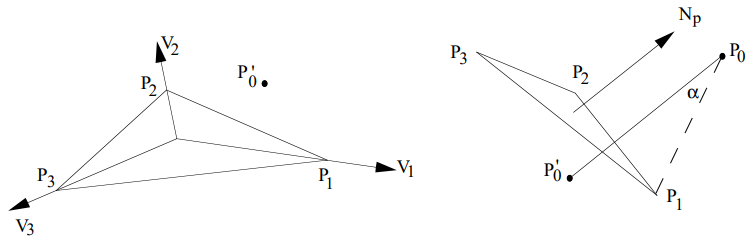
\includegraphics[width=12cm]{Images/Chap2/JonesDist.png}
    \caption{Calculating distance through projection by Jones\cite{jones19953d}}
    \label{br:jonesproj}
\end{figure}

\hspace*{\fill}

Eberly \cite{eberly2008distance} introduced a computation solution that uses the vector technique. He parameterized the triangles $ \mathbf{T}(s, t) $ as the weighted sum of two edges and a point as formula \ref{br:elberTri}:

\begin{equation}
    \mathbf{T}(s, t)=\mathbf{B}+s \mathbf{E}_{0}+t \mathbf{E}_{1}
    \label{br:elberTri}
\end{equation}

for $(s, t) \in D=\{(s, t): s \geq 0, t \geq 0, s+t \leq 1\}$, then the shortest distance can be found through calculate the minimal value of the function \ref{br:elberTriFunc}:

\begin{equation}
    \mathbf{Q}(s, t)=|\mathbf{T}(s, t)-\mathbf{P}|^{2}
    \label{br:elberTriFunc}
\end{equation}

Ericson \cite{ericson2004real} applied the Barycentric coordinates of the triangles to compute the distance. This author's method computes the distance by calculating the barycentric coordinates of point P first and then testing which Voronoi region does the projection of p located to compute the distance.

\begin{figure}[htbp]
    \centering
    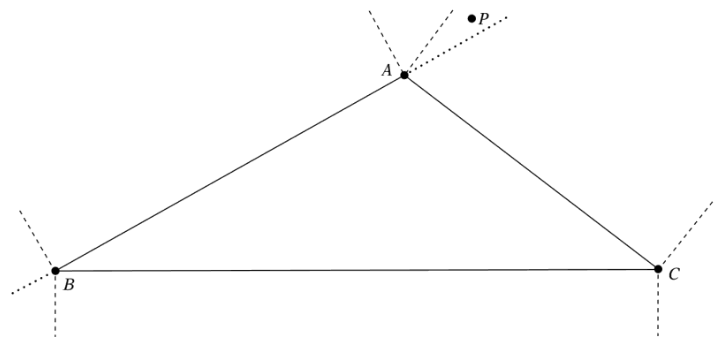
\includegraphics[width=10cm]{Images/Chap2/Barycentric.png}
    \caption{The situation of point p's projection lies on Voronoi region CA when ABC is a obtuse triangle that introduced in Ericson \cite{ericson2004real}'s paper.}
\end{figure}

Ray tracing is also a direction for solving the triangle distance problem. Tomas Akenine-M{\"o}ller and Ben Trumbore \cite{AkenineMller2005FastMS} introduced a solution which avoids pre-compute whether the ray intersects with the triangle plane. This method can compute the distance value through matrix manipulation rather than square root computation.

\subsubsection{Sign Function Computation}

Payne and Toga \cite{payne1992sdf} introduced a basic method for sign computation through scanning. The dot product of surface normal $\vec{n} $ and direction vector $ \vec{d} $ can be used to test the interior or exterior problem. However, they also noticed that this method is not always working for $ C^{1} $ discontinuous surfaces, which is the property of most polygonal meshes.

\hspace*{\fill}

An alternative is to replace the surface-normal with angle weighted pseudo-normal, which was introduced by Baerentzen and Aanaes \cite{awpseuNormal} in 2005. They first extend the angle weighted pseudo-normal of vertices introduced by Thürrner and Wüthrich\cite{awpnfirst} to edges and faces, then applied the upgraded method to the signed function computation algorithm. However, Xu and Barbi\v{c} \cite{XuagpnSlow} observed that this approach did not improve the efficiency of their research.

\hspace*{\fill}

The ray tracing method \cite{AkenineMller2005FastMS} mentioned in \ref{br:dfc} also provide a solution for testing the direction of ray and triangle intersection. If we use this method to compute the distance, then the result of normal can be reused during the sign judgement process.

\subsection{Algorithms}
\label{br:algorithm2}

After calculating the signed distance for a single triangle, the problem becomes how to compute oriental distance values for point sets.

\hspace*{\fill}

Payne and Toga \cite{payne1992sdf} introduced the naive or brutal-force method, which simply computes distances for all points in the space. The pseudo-code is shown as Algorithm \ref{br:bfalgo}:

\begin{algorithm}[H]
    \caption{Brutal Force SDF generation}
    \label{br:bfalgo}
    \begin{algorithmic}

    \For{each point(x,y,z)}
        \State $ dist=\infty $
        \For{ = each triangle t}
        \State $ newdist = distance_to_triangle(point, t) $
        \If{abs(newdist)<abs(dist)}
            \State $ dist = newdist $
        \EndIf
        \EndFor
    \EndFor

    \end{algorithmic}
\end{algorithm}

Inigo Quilez, the developer of ShaderToy \cite{shadertoy} published the SDF calculation method for most of the basic geometric shapes like Boxes and Capsules \cite{IQSDF}, but decomposing the arbitrary objects into fundamental shapes is not realistic.

\hspace*{\fill}

Both Frisken et al. \cite{frisken2000sample}, and \cite{Ju2004sample}'s researches used the sampling method to generate the signed distance without computing every triangle. For this project, it can be a potential solution. Specifically, the testing can be used through the ray intersection test. A number of equally distributed sample rays should be generated for a single sample grid to test the intersection with models. Regarding the grid as a sphere, the sample ray can be generated by dividing the sphere equally, Ahn \cite{glsphere} provided a method to calculate the coordinates of arbitrary points on the sphere by splitting the sphere. This method can be used to generate the sample rays for any direction.

\hspace*{\fill}

Building SDF for objects is time-consuming, especially when the object has a large number of triangles. Fortunately, as for a similar technique, ray tracing, the solution for the same problem has been explored for a long time and can apply to the signed distance field.

\hspace*{\fill}

To reduce the count of the traverse, we need to reduce the range of computing. Bounding volume is a widespread solution. There are several choices for constructing a bounding volume for three-dimensional meshes. The bounding sphere is the most simple choice. However, using a sphere as a bounding volume is usually unbefitting for three-dimensional objects. The distance computing through the bounding sphere contains expensive square root computation to reduce the efficiency \cite{Sanchez2012EfficientEO}. The Axis-aligned bounding box (AABB) has developed research, which is widely used for ray tracing\cite{Havran2000HeuristicRS}. This structure has a good balance of generation time and quality. Therefore, AABB is the most popular choice for acceleration \cite{Sanchez2012EfficientEO}.

 \begin{figure}[htbp]
    \centering
    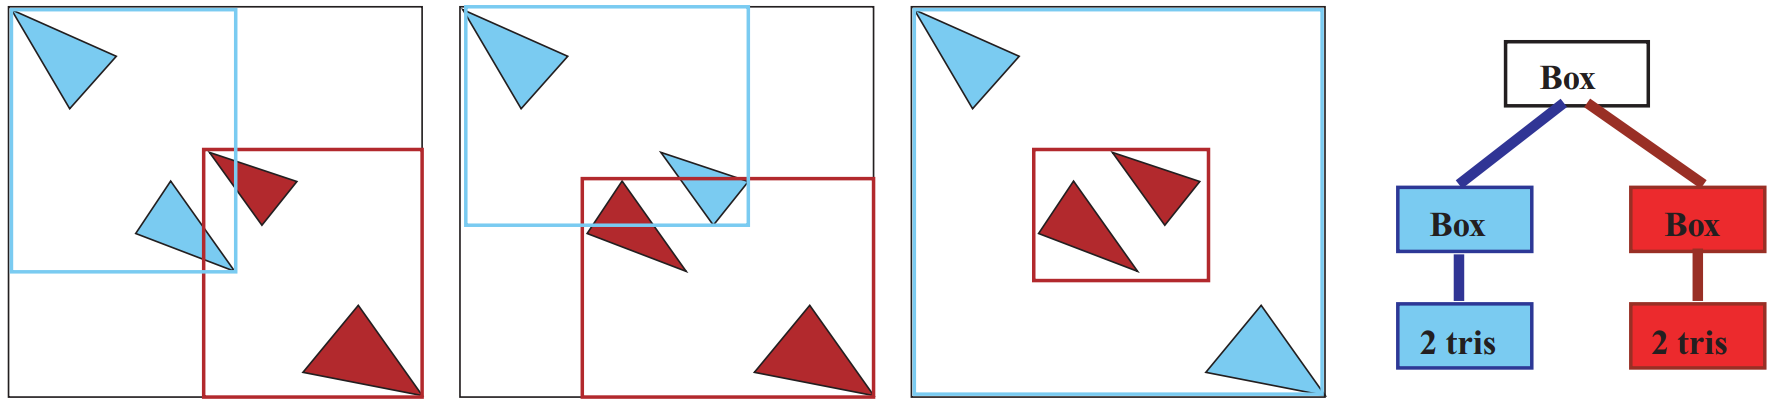
\includegraphics[width=16cm]{Images/Chap2/BVH.png}
    \caption{Different BVHs for 4 triangles provided by Wald \cite{bvhraytracing}}
    \label{br:bvh}
 \end{figure}

 Similarly, the acceleration structure for ray tracing can be extended to SDF computation. There are two primary tree-structured options: Bounding Volume Hierarchy (BVH) and K-dimensional Tree, representing two different solutions directions.

\hspace*{\fill}

 BVH split the whole object according to its primitives, for this project, triangles. Wald \cite{bvhraytracing} gives a brief explanation of BVH in his research. When building a BVH, it is recursively creating newer and smaller bounding volumes according to the size of primitives for every children node; as a result, the edge of children nodes' bounding volume can be different from its parent. Each leaf node store the bounding volume for different primitives. Ideally, different primitives will only be saved to one single leaf node and can be traversed through parent nodes. Strategies for building BVH are illustrated in figure \ref{br:bvh}.

\hspace*{\fill}

The principle of the KD-tree building is similar to BVH, except the method of splitting the space is different. The KD-tree structure is mostly built using AABB bounding volume \cite{kdraytracing}. Building a KD tree for space will recursively divide the whole space with the position of primitives alongside the axis. The bounding box of the children nodes must share some edges with its parent nodes. When ray tracing through the KD-tree structure, the algorithm will test whether the ray intersects with the bounding box. If a ray only intersects one side of a box, then the ray must shoot on a primitive contained in the box node; the traverse will continue until the correct leaf node is found \cite{kdraytracing}. In the comparison of Havran\cite{Havran2000HeuristicRS}, this structure is the best method for CPU implementation. As for SDF generation, Inigo Quilez has a WebGL implementation on ShaderToy \cite{kdtoy}, which proved that the solution fits the requirement of SDF computation. An example given by Foley \cite{kdraytracing} of KD-tree ray tracing showed in figure \ref{br:kd}. 

\begin{figure}[htbp]
    \centering
    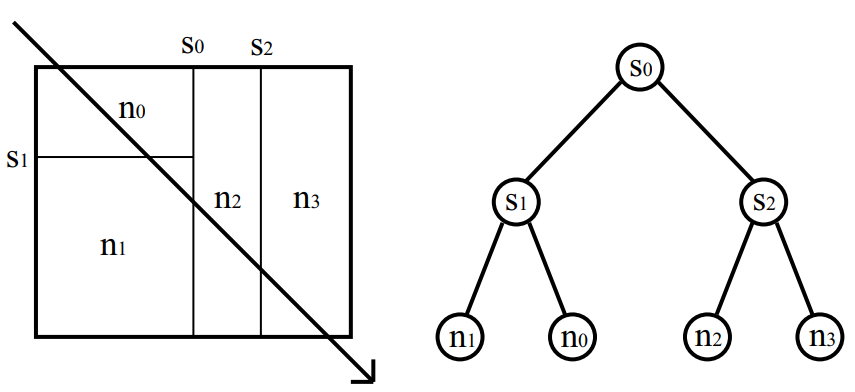
\includegraphics[width=14cm]{Images/Chap2/kd.png}
    \caption{Left: The principle of kd-tree ray tracing. Right:The structure of the same tree}
    \label{br:kd}
\end{figure}


\subsection{Technologies and Tools}
\label{br:tt}

\subsubsection{Graphics APIs}
\label{br:api}

In computer graphics, the Graphics Application Programming Interface, or Graphics API, plays a vital role in determining how the GPU manipulate the rendering tasks. For the graphics programmers, a friendly API will increase the development efficiency.

\hspace*{\fill}

Three Graphics APIs are widely used: OpenGL, Vulkan and Direct3D.

\paragraph{OpenGL}

Open Graphic Library or OpenGL \cite{OpenGLofficial}, is a cross-platform and language-independent Graphics API, which was initially developed by Silicon Graphics, Inc. (SGI) \cite{kessenich2016opengl}. Khronos Group has continued to manage the development of this API since 2006. Its Version 1.0 was released in July of 1994, and the latest version was updated to 4.6. OpenGL is able to render both 2D images, and 3D graphics through a graphics processing unit (GPU) \cite{kessenich2016opengl}. Although C++ is the most chosen programming language for developing OpenGL applications, using JavaScript, C and Java to create OpenGL applications on IOS, Android or web browsers are available.

\paragraph{Direc3D}

Direct3D \cite{d3dofficial} is the main competitor of OpenGL and Vulkan created by Microsoft. It only runs on Microsoft environments like Windows, Xbox and UWP applications. As a low-overhead Graphics API, Direct3D allows the programmer to control synchronization and multi-threading; compared with standard APIs, it has higher efficiency and saves more resources \cite{d3d10} \cite{blythe2006direct3d}.

\paragraph{Vulkan}

Vulkan is the newest Graphics API, which was developed by Khronos Group and first released in February of 2016. Vulkan was positioned as the successor of OpenGL, it keeps cross-platform capabilities and aims to create the graphic applications with complex, and numerous datasets \cite{sellers2016vulkan}. Therefore, Vulkan will be widely used in industry in the future. Vulkan gives the programmer a high degree of freedom during the development process; the responsibility of synchronization, scheduling or memory management and many other features belongs to the programmer, which also means that compared with OpenGL, Vulkan gives higher requirements on the experience for application writers \cite{sellers2016vulkan}.

\subsubsection{Languages}

\paragraph{C++}

C++ is a general-purpose programming language based on the C programming language \cite{c++iso}, developed by Bjarne Stroustrup and released in 1985 \cite{Stroustrup1997}. C++ is widely used in the graphics industry. All of the Graphics APIs mentioned in \ref{br:api} provide support for C++, and Vulkan only officially provides C++ wrapper support since the property of memory management.

\paragraph{Python}

Python \cite{pythonoffcial} is a popular interpreted, general-purpose programming language developed by Guido van Rossum around 1990 \cite{lutz2001programming}. With the development of deep learning, many popular and friendly python frameworks and libraries have been created. For example, TensorFlow \cite{TensorFlow} and Keras \cite{Keras}. There are already successful examples applying Deep Learning technology to graphics like NVIDIA's DLSS (Deep Learning Super Sampling) \cite{DLSS}. Moreover, as mentioned in \ref{br:3dsdf}, the research of Park \cite{park2019deepsdf} about signed distance field was based on deep learning technology.

\subsubsection{Graphical User Interface libraries}

\paragraph{GLFW}

GLFW \cite{glfw} is a cross-platform C library for OpenGL, OpenGL ES and Vulkan. This library allows programmers to create and handle application windows, contexts and surfaces, user input and many other functions.

\paragraph{ImGui}

Dear ImGui \cite{dearimgui} is a open-source C++ graphical user interface library developed by Omar Cornut. The core source code of Dear ImGui is only contained in several platform-independent files. Therefore, it is portable and easy to be compiled with other application codes. Most of the mainstream Graphics APIs, including DirectX, OpenGL, Vulkan, and platforms including Windows, OSX are supported. Dear ImGui also provides useful extensions, including Text Editors and Animation Editors.

\paragraph{Qt}

Qt \cite{qt} is a robust cross-platform UI framework for C++ \cite{sherriff2018qt}, which was initially developed by Haavard Nord and Eirik Chambe-Eng in 1990, and the responsibility of development belongs to The Qt Company. Qt provides a series of tool kits for UI development, including declarative language QML \cite{qml}, compilation tool qmake \cite{qmake} and an integrated development environment (IDE) Qt Creator \cite{qtcreator}. The programmer is able to create a complete application only in Qt environment. 

\subsubsection{Building Project}

\paragraph{Premake}
\label{premake}

Premake \cite{premake} is open-source utility software for source code building. Lua \cite{lua} Script is used for premake to store the information of software projects. Premake use the command line to read the project configuration for different platforms from a Script and generate project of development IDEs 

\paragraph{CMake}

CMake \cite{cmake} is an open-source compiler-independent for source code building, testing and packaging. It is mostly used for C and C++ languages. A C++ compiler like MinGW is necessary for project building. CMake also supports mainstream IDEs like Visual Studio and Xcode.

\subsubsection{Model file formats}

\paragraph{OBJ}

OBJ \cite{OBJ} file is a geometry file format developed by Wavefront Technologies for its Advanced Visualizer animation tool. This format contains the positions of vertices, UV mapping information, vertex normals and the list of each polygon face. OBJ files store the information of vertex in counter-clockwise order. Wavefront Technologies also developed the Material Template Library (MTL) format for OBJ to store the material properties of objects.

\paragraph{FBX}

FBX (FilmBox) \cite{FBX} is a file format for 3D models, which was initially developed by Kaydara for MotionBuilder and owned by Autodesk in 2006. FBX file is a tree-structured document and can be used for animation by storing the motion nodes.


\section{Choice of Methods}

\subsection{Choice of Method and Algorithm}
\label{br:cAlgo}

Considering about the difficulty of implementation and time limitation, several methods and algorithms are chosen for this project. 

\hspace*{\fill}

First, the field generation method is sampling the points in a limited bounding box range and calculating the distance values for them through a number of sample rays; when setting the appropriate parameters (e.g. resolution, number of sample rays), we can get a satisfying result. Second, the chosen method of computing signed distance values is the ray tracing solution \cite{AkenineMller2005FastMS} mentioned in \ref{br:dfc}, because this method solves the distance function computation problem through matrix rather than square root computation, which will get the exact value with relatively low consumption. Then, the acceleration strategy is applied KD-tree data structure alongside the AABB bounding volume during the process of constructing the signed distance field, which is a widely used space acceleration structure; the successful commercial game engine Unreal Engine uses this structure to generate SDF \cite{uesdf}. Finally, using multi-threading programming to improve efficiency. Undoubtedly, GPU implementation is a better way for acceleration for generating SDF. However, the HPG courses are not cover related content like CUDA programming; therefore, GPU implementation will be a tricky method for this project and may result in the project not being completed on time. Besides, avoiding GPU implementation brings better compatibility since there will be no requirement for specific hardware.

\subsection{Choice of Technologies}
\label{br:ctpl}

\subsubsection{Language and Graphics API}

The libraries, frameworks and APIs mentioned in \ref{br:tt} provide support for C++. Besides, the compatibility and efficiency of C++ satisfied the requirement of Graphics application development. Therefore, C++ becomes the chosen language for this project.

\hspace*{\fill}

OpenGL and Vulkan are covered by High-Performance Graphics and Games Engineering MSc modules, while Direct3D is not. Direct3D obviously is a risky option. Besides, considering the time limitation and the requirement of Vulkan API, OpenGL becomes the final chosen API for this project because of its compatibility and relatively easy to implement.

\hspace*{\fill}

A review of the OpenGL graphics pipeline is helpful for further application design.

\hspace*{\fill}

As shown in figure \ref{br:pipeline} \cite{learopengl}, the pipeline is divided into several stages; each stage will collect the output data from its last stage and process the data for the next.

The first stage is named Vertex Specification. Two concepts should be cleared before continuing to introduce the pipeline. Vertex Buffer Objects (VBO) are the buffers containing a number of information (e.g. positions, normals, colours) of vertices in video memory \cite{vetspeci}. Vertex Array Object (VAO) contains at least one VBO as well as the definition of vertex data \cite{vetspeci}. The GPU use VAO and VBO to analyze the vertex data for rendering.

\paragraph{Vertex Shader}

Vertex Shader is a programmable stage which can be used to process the attributes of vertex \cite{vetsha}. The vertex shader is mostly used to make transformations of coordinates for vertex data, including local-world transformation, view transformation and clipping. Tessellation \cite{tesse} and Geometry Shader \cite{gs} are two optional stages; the former can divide data into smaller primitives, while the latter can modify the input to geometric shapes like triangles.

\paragraph{Primitive Assembly}

Primitive Assembly \cite{pa} aims to modify the former primitives to a sequence of basic primitives like lines. When Tessellation or Geometry Shader is active, an early primitive assembly process will happen before both \cite{vetsha}.

\paragraph{Rasterisation}

Then it comes to Rasterisation \cite{pipeall}. The output of Primitive Assembly is primitives; they will be processed to screen position by perspective and viewport transformation. The output of this stage is screen coordinates, to be specific, the position of pixels. Those pixels (fragments) will be sent to the fragment shader for colour computation in the next stage.

\paragraph{Fragment Process}

Fragment Process \cite{pipeall} is another programmable stage of the pipeline. Colours, depth values and possible stencil values will be computed in Fragment Shader \cite{fs} and set as the output of this shader, which will be passed to the final testing and blending stage \cite{psp} , where the scissor test, alpha test and depth test will happen. Finally, the data will be passed to the framebuffer and shown on the screen.

\subsubsection{GUI}

The user interface of the final application only needs a panel to show buttons, checkboxes and text information. Considering the complexity of setting up the development environment and writing Qt code, using Qt is too obese for this project. Dear ImGui is enough to implement the features mentioned above and can also avoid the potential problems caused by different Qt environments. Therefore, the project will be developed through Dear ImGui.

\hspace*{\fill}

Without Qt, the only option for application window control API is GLFW. Finally, the GUI will be created through GLFW alongside Dear ImGui.

\subsubsection{Building Project}
\label{premake2}

To generate a project through CMake, the user must install and set the appropriate environment for this tool kit. However, some potential problems will happen in specific situations, like the version differences on different devices. Compared with CMake, Premake only needs to define the configuration of the project when creating Lua script, which also enhances the understanding of project structure. Therefore, this project chose Premake as the tool for building project.

\subsubsection{Model file formats}
\label{br:cmf}

There is no requirement to make animation for the project; the OBJ file satisfies the load test models' demand and becomes the chosen format.

\subsubsection{Third Party Libraries}

Moreover, some third-party libraries help implement the application. An OpenGL Loading Library is used to load the pointers to OpenGL functions. The project chose glad \cite{glad} as the final option of this library because of a similar reason to choosing Dear ImGui. For mathematics and model load libraries, the situations are analogical; there is one widely used library for each field with no obvious alternative solutions, GLM \cite{glm} (for mathematics), and tinyobjloader \cite{objload} (for loading obj file). Therefore, they become the chosen third-party libraries.